% !TEX TS-program = pdflatex
\documentclass[aspectratio=169]{beamer}
\usepackage[utf8]{inputenc}
\usepackage[T1]{fontenc}
\usetheme{Madrid}
\usecolortheme{seahorse}
\usefonttheme{professionalfonts}
\setbeamertemplate{navigation symbols}{}
\setbeamercovered{transparent}
\setbeamertemplate{itemize items}[circle]
\setbeamertemplate{enumerate items}[default]
\setlength{\parskip}{0.15em}

\definecolor{bepurple}{RGB}{107,63,160}
\definecolor{begold}{RGB}{200,168,75}
\definecolor{beteal}{RGB}{26,122,110}
\definecolor{berust}{RGB}{192,68,42}
\definecolor{beblue}{RGB}{26,74,138}
\definecolor{softpurple}{RGB}{240,232,255}
\definecolor{softgold}{RGB}{255,248,220}
\definecolor{softteal}{RGB}{220,242,240}
\definecolor{softrust}{RGB}{255,235,230}
\setbeamercolor{structure}{fg=beblue}
\setbeamercolor{title}{fg=white,bg=beblue}
\setbeamercolor{frametitle}{fg=beblue}
% Minimal block rendering: regular/example blocks become colored headings (no box)
\setbeamertemplate{block begin}{%
  \par\vspace{0.2ex}%
  \ifx\insertblocktitle\empty\else%
    {\usebeamerfont{block title}\color{beblue}\textbf{\insertblocktitle}}\par\vspace{0.2ex}%
  \fi%
}
\setbeamertemplate{block end}{\par\vspace{0.2ex}}
\setbeamertemplate{block example begin}{%
  \par\vspace{0.2ex}%
  \ifx\insertblocktitle\empty\else%
    {\usebeamerfont{block title}\color{beteal}\textbf{\insertblocktitle}}\par\vspace{0.2ex}%
  \fi%
}
\setbeamertemplate{block example end}{\par\vspace{0.2ex}}
\setbeamertemplate{block alerted begin}{%
  \par\vspace{0.5ex}%
  \begin{beamercolorbox}[sep=0.5ex,rounded=true,shadow=false]{block title alerted}%
    \usebeamerfont{block title}\insertblocktitle%
  \end{beamercolorbox}%
  \nointerlineskip%
  \begin{beamercolorbox}[sep=0.5ex,rounded=true,shadow=false]{block body alerted}%
    \usebeamerfont{block body}%
}
\setbeamertemplate{block alerted end}{\end{beamercolorbox}\par\vspace{0.5ex}}
\setbeamercolor{block title alerted}{fg=white,bg=berust}
\setbeamercolor{block body alerted}{fg=black,bg=berust!8}
\setbeamercolor{alerted text}{fg=berust}

\usepackage{booktabs,amsmath,amssymb,array,multirow,hyperref,colortbl,xcolor}
\usepackage{tikz}
\usepackage{pgfplots}
\pgfplotsset{compat=1.18}
\usetikzlibrary{arrows.meta,positioning,calc,shapes.geometric,patterns,trees}
\hypersetup{colorlinks=true,linkcolor=beblue,urlcolor=beblue}

\title{\textbf{Lecture 7: Behavioural Game Theory}}
\subtitle{Level-k Thinking, the Beauty Contest, and Why Nash Equilibrium Often Fails}
\author{Prof.\ Muhebullah Karimzada}
\institute{School of Economics, University of Northern British Columbia}
\date{ECON 230 $\cdot$ Introduction to Behavioural Economics $\cdot$ Winter 2027}

\begin{document}

\begin{frame}[plain]\titlepage\end{frame}

% ============================================================
\begin{frame}{[GAME] The Beauty Contest --- Play Now!}
\note{CRITICAL: collect answers BEFORE any discussion. Write a number between 0 and 100 on a piece of paper. Do NOT discuss with neighbors. Calculate the average after collecting, then compute 2/3 of average, announce winner.}
\begin{alertblock}{The Keynesian Beauty Contest}
\textbf{Guess a number between 0 and 100.}\\[0.3em]
The winner is the person whose guess is \textbf{closest to $\frac{2}{3}$ of the average guess} across all players.\\[0.4em]
\textit{Write your answer on a piece of paper. Do not discuss with neighbours. Hand it to the front.}
\end{alertblock}
\begin{block}{Why ``Beauty Contest''?}
Keynes (1936) described stock market investing as a beauty contest where you don't pick who \textit{you} find most beautiful, but who you think \textit{others} will find most beautiful. The same logic applies here: don't guess what \textit{you} think is right --- guess what you think others will guess (times 2/3).
\end{block}
\end{frame}

% ============================================================
\begin{frame}{Lecture Overview}
\begin{enumerate}[<+->]
  \item \textbf{Nash equilibrium} and what it requires
  \item \textbf{Level-k thinking} --- strategic reasoning in steps
  \item \textbf{Beauty Contest debrief} --- where does your class cluster?
  \item \textbf{The Centipede Game} --- backward induction failures
  \item \textbf{The Prisoner's Dilemma} --- cooperation vs defection
  \item \textbf{Repeated games and cooperation} --- Folk Theorem, Tit-for-Tat
  \item \textbf{Quantal Response Equilibrium} --- noisy best responses
  \item \textbf{Applications:} auctions, oligopoly, negotiations
\end{enumerate}
\end{frame}

% ============================================================
\section{Nash Equilibrium Revisited}
% ============================================================

\begin{frame}{Nash Equilibrium --- What It Actually Requires}
\begin{block}{Definition}
A strategy profile $(s_1^*, \ldots, s_n^*)$ is a Nash Equilibrium if no player can unilaterally improve their payoff by deviating.
\end{block}
\begin{columns}
\column{0.5\textwidth}
\begin{alertblock}{What Nash Equilibrium Requires}
\begin{enumerate}
  \item Everyone is \textbf{rational}.
  \item Everyone knows that everyone is rational.
  \item Everyone knows that everyone knows that everyone is rational.
  \item \textit{Ad infinitum.} This is \alert{Common Knowledge of Rationality (CKR)}.
\end{enumerate}
\textbf{This is an extremely strong assumption.}
\end{alertblock}
\column{0.47\textwidth}
\begin{exampleblock}{The Empirical Failure}
CKR fails whenever:
\begin{itemize}
  \item Players have limited depths of reasoning (most people: 1--2 steps)
  \item Players have social preferences (Lecture 6)
  \item Players have bounded rationality (Lecture 1)
  \item The game is unfamiliar
\end{itemize}
\textbf{Nash equilibrium is a long-run benchmark}, not a description of initial play.
\end{exampleblock}
\end{columns}
\end{frame}

% ============================================================
\begin{frame}{The Prisoner's Dilemma}
\begin{columns}
\column{0.47\textwidth}
\begin{block}{The Game}
\begin{center}
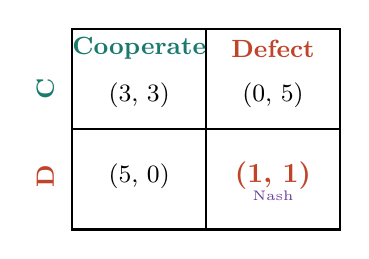
\begin{tikzpicture}[scale=0.85]
\draw[thick] (0,0) rectangle (4,3);
\draw[thick] (2,0) -- (2,3);
\draw[thick] (0,1.5) -- (4,1.5);
\node[font=\small\bfseries,beteal] at (1,2.7) {Cooperate};
\node[font=\small\bfseries,berust] at (3,2.7) {Defect};
\node[font=\small\bfseries,beteal,rotate=90] at (-0.4,2.1) {C};
\node[font=\small\bfseries,berust,rotate=90] at (-0.4,0.8) {D};
\node[font=\small] at (1,2.0) {(3, 3)};
\node[font=\small] at (3,2.0) {(0, 5)};
\node[font=\small] at (1,0.8) {(5, 0)};
\node[font=\small,berust,font=\bfseries] at (3,0.8) {(1, 1)};
\node[font=\tiny,bepurple] at (3,0.5) {Nash};
\end{tikzpicture}
\end{center}
\end{block}
\column{0.5\textwidth}
\begin{block}{Analysis}
\begin{itemize}
  \item D \textbf{dominates} C for both players.
  \item Nash: (D,D) --- both get \textbf{1}.
  \item Pareto optimum: (C,C) --- both get \textbf{3}.
  \item Cooperation is \textit{not} a Nash equilibrium in a one-shot game.
\end{itemize}
\end{block}
\begin{alertblock}{Real-World PDs}
\begin{itemize}\small
  \item Airline price wars; OPEC cartel
  \item Nuclear arms races; advertising wars
  \item Antibiotic resistance; climate change
\end{itemize}
\end{alertblock}
\end{columns}
\end{frame}

% ============================================================
\begin{frame}{[GAME] Prisoner's Dilemma in Class}
\note{Pair students. Play 5 rounds with SAME partner (results revealed each round). Then play with new partner. Observe how cooperation evolves. Key lesson: cooperation can emerge in repeated games even among strangers.}
\begin{block}{Rules}
\begin{enumerate}
  \item Pair with your neighbour. You will play 5 rounds with the \textbf{same} partner.
  \item Each round: simultaneously write \textbf{C} (cooperate) or \textbf{D} (defect).
  \item Payoffs: (C,C) = (3,3). (C,D) = (0,5). (D,C) = (5,0). (D,D) = (1,1).
  \item Reveal after each round. Keep a running score.
\end{enumerate}
\end{block}
\begin{block}{Debrief Questions}
\begin{itemize}
  \item How many pairs ended up at (C,C)? (D,D)?
  \item Did strategy evolve over the 5 rounds?
  \item Did you use Tit-for-Tat? Did it work?
  \item How did it feel to be defected on after cooperating?
\end{itemize}
\end{block}
\end{frame}

% ============================================================
\section{Level-k Thinking}
% ============================================================

\begin{frame}{The Level-k Model}
\textcolor{beblue}{\textbf{Stahl \& Wilson (1994); Nagel (1995):}} Instead of CKR (infinite depth), players have types by \textbf{reasoning depth}:
\begin{columns}
\column{0.5\textwidth}
\textcolor{beblue}{\textbf{Level Types:}}
\begin{itemize}\small
  \item \textbf{L0:} Uniform random or non-strategic.
  \item \textbf{L1:} Best respond to L0 belief.
  \item \textbf{L2:} Best respond to L1 belief.
  \item \textbf{Nash:} $k \to \infty$.
\end{itemize}
\column{0.47\textwidth}
\textcolor{beblue}{\textbf{Beauty Contest:}}
\begin{itemize}\small
  \item \textbf{L0} plays \textbf{50}. \textbf{L1} plays \textbf{33}. \textbf{L2} plays \textbf{22}.
  \item \textbf{L3:} 15. \textbf{L4:} 10. \textbf{Nash:} 0.
\end{itemize}
\end{columns}
\begin{alertblock}{What Empirical Data Shows}
Spikes at 33 (L1) and 22 (L2). Few at 0. \textbf{Most people are L1--L2.} FT competition (1,500 readers): winning guess = 13 ($\approx$L3). Camerer et al.\ (2004): average $k \approx 1.5$.
\end{alertblock}
\end{frame}

% ============================================================
\begin{frame}{Beauty Contest Debrief --- Your Class Results}
Compute: (1) class average; (2) $\frac{2}{3}\times$ average; (3) find the winner; (4) plot distribution.
\begin{columns}
\column{0.5\textwidth}
\begin{exampleblock}{Nagel (1995) Data}
\begin{itemize}\small
  \item Caltech: mean $\approx$34 (L1). Grad students: $\approx$25 (L2).
  \item FT competition (1,500 readers): 13.
  \item Science readers (Germany): $\approx$22.
\end{itemize}
\end{exampleblock}
\column{0.47\textwidth}
\begin{tikzpicture}
\begin{axis}[
  width=\textwidth,height=0.6\textheight,
  xlabel={\small Guess},ylabel={\small Frequency (\%)},
  xmin=0,xmax=100,ymin=0,ymax=25,
  axis lines=left,
  title={\small Typical Beauty Contest Distribution}
]
\addplot[beblue,ybar,bar width=4pt,fill=beblue!50] coordinates{
  (5,2)(10,3)(15,4)(20,7)(25,8)(30,12)(33,18)(35,10)(40,8)
  (45,5)(50,16)(60,5)(67,3)(75,3)(100,4)
};
\draw[dashed,berust] (axis cs:33,0) -- (axis cs:33,22) node[above,font=\tiny,berust]{L1};
\draw[dashed,beteal] (axis cs:22,0) -- (axis cs:22,10) node[above,font=\tiny,beteal]{L2};
\node[font=\tiny,bepurple] at (axis cs:5,21){Nash=0};
\end{axis}
\end{tikzpicture}
\end{columns}
\end{frame}

% ============================================================
\begin{frame}{The Centipede Game}
\begin{block}{Rosenthal (1981)}
Two players alternate moves. At each node: \textbf{Take} (game ends, payoffs as below) or \textbf{Pass} (game continues, pot doubles). Standard backward induction: Player 1 should Take at node 1!
\end{block}
\begin{center}
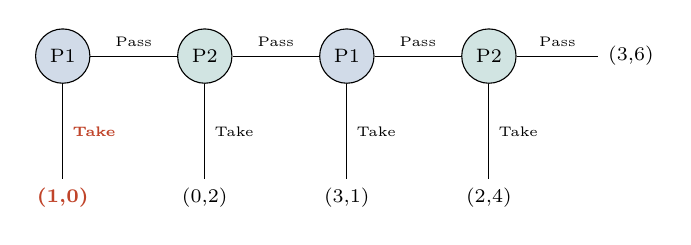
\begin{tikzpicture}[scale=0.82,
  level 1/.style={level distance=2.2cm,sibling distance=1.2cm}]
\node[circle,draw,fill=beblue!20,font=\scriptsize] (n1) {P1}
  child[grow=right] {
    node[circle,draw,fill=beteal!20,font=\scriptsize] (n2) {P2}
      child[grow=right] {
        node[circle,draw,fill=beblue!20,font=\scriptsize] (n3) {P1}
          child[grow=right] {
            node[circle,draw,fill=beteal!20,font=\scriptsize] (n4) {P2}
              child[grow=right] { node[font=\scriptsize] {(3,6)} edge from parent node[above,font=\tiny]{Pass} }
              child[grow=south] { node[font=\scriptsize] {(2,4)} edge from parent node[right,font=\tiny]{Take} }
            edge from parent node[above,font=\tiny]{Pass}
          }
          child[grow=south] { node[font=\scriptsize] {(3,1)} edge from parent node[right,font=\tiny]{Take} }
        edge from parent node[above,font=\tiny]{Pass}
      }
      child[grow=south] { node[font=\scriptsize] {(0,2)} edge from parent node[right,font=\tiny]{Take} }
    edge from parent node[above,font=\tiny]{Pass}
  }
  child[grow=south] { node[font=\scriptsize,berust] {\textbf{(1,0)}} edge from parent node[right,font=\tiny,berust]{\textbf{Take}} };
\end{tikzpicture}
\end{center}
\begin{alertblock}{The Prediction vs Reality}
\textbf{Nash:} Player 1 takes immediately $\Rightarrow$ both get (1,0).\\
\textbf{Reality (McKelvey \& Palfrey, 1992):} Games almost \textit{never} end at node 1. Most go to node 3 or 4. Why? Social preferences, bounded rationality, level-k reasoning.
\end{alertblock}
\end{frame}

% ============================================================
\begin{frame}{Cooperation in Repeated Games}
\begin{block}{The Folk Theorem}
In an infinitely repeated game, any feasible, individually rational payoff can be sustained as a Nash Equilibrium with sufficiently patient players ($\delta$ close enough to 1). This includes the cooperative (C,C) outcome!
\end{block}
\begin{columns}
\column{0.5\textwidth}
\begin{exampleblock}{Tit-for-Tat (Axelrod, 1984)}
Robert Axelrod ran computer tournaments where strategies competed in repeated PD. \textbf{Winner (twice): Tit-for-Tat.}
\begin{itemize}
  \item \textbf{Nice:} Cooperate on round 1.
  \item \textbf{Retaliatory:} Copy opponent's last move.
  \item \textbf{Forgiving:} Return to C if opponent returns to C.
  \item \textbf{Clear:} Simple to understand.
\end{itemize}
\end{exampleblock}
\column{0.47\textwidth}
\begin{block}{Real-World Cooperation}
\begin{itemize}
  \item \textbf{OPEC:} Repeated interaction + monitoring sustains cartel.
  \item \textbf{Canada-US trade:} 150 years of largely cooperative relationship.
  \item \textbf{Indigenous ROSCAs:} Rotating savings groups in immigrant communities.
  \item \textbf{Biology:} Bacteria cooperate in biofilms despite defection incentives.
\end{itemize}
\end{block}
\end{columns}
\end{frame}

% ============================================================
\begin{frame}{Quantal Response Equilibrium}
\begin{block}{McKelvey \& Palfrey (1995)}
Instead of fully rational choice (always pick best response), players choose better options \textbf{more often but not always}:
\[
  \Pr(\text{action } a) \propto \exp(\lambda \cdot EU(a))
\]
\begin{itemize}\setlength{\itemsep}{0pt}
  \item $\lambda = 0$: Uniform random (fully irrational)
  \item $\lambda \to \infty$: Nash equilibrium (fully rational best response)
  \item Intermediate $\lambda$: ``noisy best-responder''
\end{itemize}
\end{block}
\begin{exampleblock}{Why QRE Matters}
QRE fits experimental data \textbf{far better} than Nash in centipede games, coordination games, entry games, and ultimatum games.
Nash is the limit of QRE as rationality $\lambda \to \infty$ --- QRE nests Nash as a special case.
\end{exampleblock}
\end{frame}

% ============================================================
\begin{frame}{Application --- Auctions and Winner's Curse}
In a \textbf{common value auction}, the winner has the most optimistic signal --- so the true value is likely \textit{below} their estimate. The winner is \alert{cursed}.
\begin{columns}
\column{0.5\textwidth}
\begin{alertblock}{Rational Bidding}
Shade bid \textit{below} your estimate to correct for the curse. Naive bidding: overbid by 15--30\% (Kagel \& Levin, 1986).
\end{alertblock}
\column{0.47\textwidth}
\begin{exampleblock}{Real Examples}
\begin{itemize}\small
  \item \textbf{FCC auctions:} Milgrom \& Wilson (Nobel 2020).
  \item \textbf{Canadian oil sands:} Overbidding in 1970s.
  \item \textbf{Corporate M\&A:} Acquirers typically overpay.
  \item \textbf{IPOs:} Retail get what professionals reject.
\end{itemize}
\end{exampleblock}
\end{columns}
\end{frame}

% ============================================================
\begin{frame}{Discussion Questions}
\begin{enumerate}
  \item[\textcolor{bepurple}{Q1.}] ``If you were designing a government procurement auction, how would you account for winner's curse? What rules would minimise overbidding?''
  \medskip
  \item[\textcolor{beteal}{Q2.}] ``Can you think of a real-world `beauty contest' situation where being wrong in the \textit{same direction as everyone else} is safer than being right alone?'' (Hint: fund manager career concerns; housing market)
  \medskip
  \item[\textcolor{berust}{Q3.}] ``Canada's telecom market (Bell, Rogers, Telus): is this repeated-game tacit collusion, competitive equilibrium, or something else? What evidence would distinguish these?''
\end{enumerate}
\end{frame}

% ============================================================
\begin{frame}{Key Takeaways --- Lecture 7}
\begin{itemize}
  \item[\textcolor{beteal}{\checkmark}] \textbf{Nash requires CKR} --- common knowledge of rationality to infinite depth. Unrealistic.
  \item[\textcolor{beteal}{\checkmark}] \textbf{Level-k model:} L0 = random, L1 = best respond to L0, ...; most people are L1--L2.
  \item[\textcolor{beteal}{\checkmark}] \textbf{Beauty contest:} Nash = 0, typical winning guess = 13--33 depending on audience.
  \item[\textcolor{beteal}{\checkmark}] \textbf{Centipede:} backward induction fails; cooperation near start of game.
  \item[\textcolor{beteal}{\checkmark}] \textbf{Repeated games:} cooperation supported by Folk Theorem, Tit-for-Tat, social norms.
  \item[\textcolor{beteal}{\checkmark}] \textbf{QRE:} noisy best-response; nests Nash; fits data better in lab.
  \item[\textcolor{beteal}{\checkmark}] \textbf{Applications:} auctions (winner's curse), oligopoly (tacit collusion), M\&A (overbidding).
\end{itemize}
\medskip\textcolor{beblue}{\textbf{Next:}} \textbf{Lecture 8: Behavioural Finance} --- How individual biases aggregate into market bubbles, crashes, and persistent anomalies.
\end{frame}

\end{document}
